\section{Objetivos}
O objetivo principal desta prática é tanto a dedução da equação em tempo discreto de um PID, como a sua implementação prática em ambiente Simulink\textregistered e em código básico de Matlab\textregistered.

\section{Fundamentação Teórica}

\section{Procedimentos}
\subsection{Exercício 1}
Considere um sistema em malha fechada com PID T(z) sendo:

\begin{figure}[H]
	\centering
	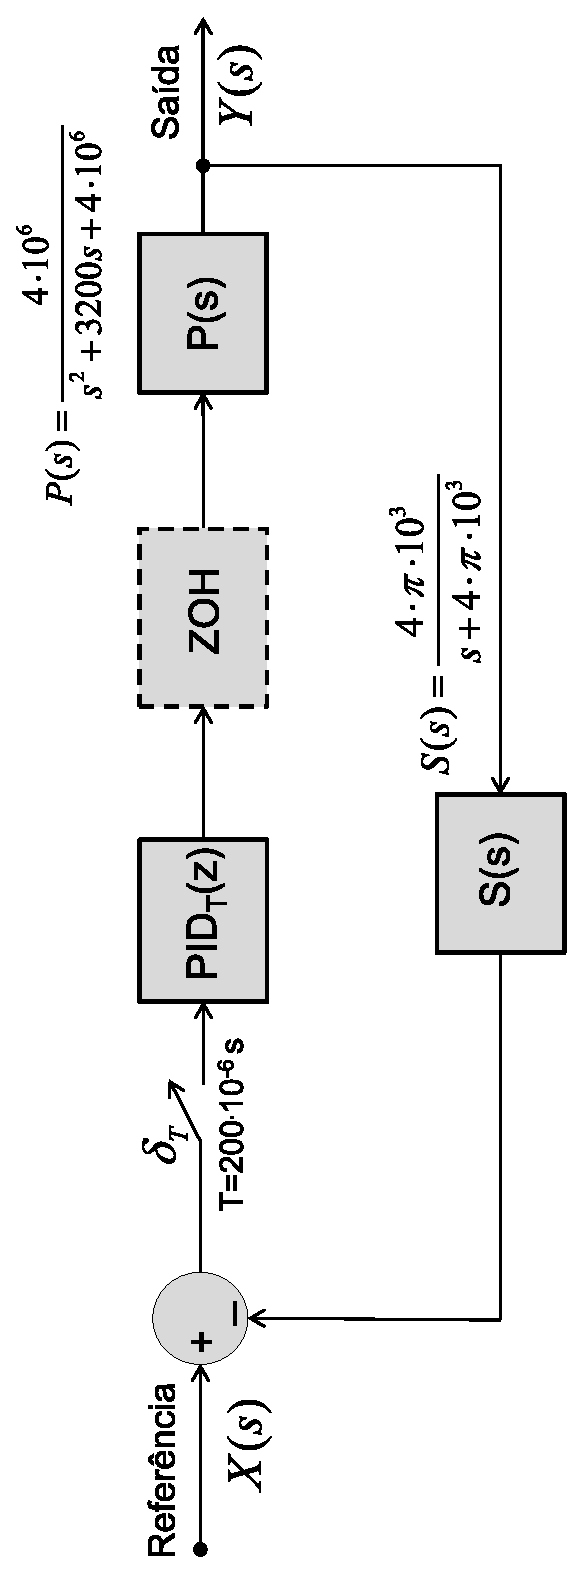
\includegraphics[scale = .5, angle =-90]{Imagens/PID.eps}
	\caption{Sistema - Exercício 1}
	\label{fig:ExercicioPID}
\end{figure}

Utilize simulações computacionais (Simulink\textregistered) para projetar ganhos para o controlador PID considerando a entrada um degrau unitário.

\subsection{Exercício 2}

Obtenha a função de transferência do PID de tempo discreto utilizando o método de discretização Forward para a parcela integral e considere Kp, Ki, e Kd como ganhos paralelos do controlador PID.

\subsubsection{Repita o Exercício 1 para esta função de transferência comparando os resultados de simulação de ambos os casos para os mesmos ganhos.}

\subsubsection{Inclua saturação na ação de controle em 150\% da referência e analise o comportamento do sistema de controle}

\subsection{Exercício 3}
Considerando o sistema descrito no exercício 2, desenvolva um script em Matlab para implementar o PID com os seguintes parâmetros.

\begin{itemize}
	\item Sinal de referência:
	Onda quadrada
	Amplitude $40~V_{pp}$
	Offset $0~V$
	Período $10ms$
	\item Controlador:
	PID ‘Digital’ (equação de diferenças)
	Saturação do PID (Sat = $0.98~V_{cc}$)
	\item Atuador: sinal PWM
	Resolução 8 bits (2n divisões)
	$V_{cc}=40~V$
	\item Ruído:
	Randômico
	Amplitude 2\% da saída
	\item Conversor A/D:
	Resolução 10 bits (2n níveis)
	Vin=0-5V
	T=200.10-6 s
	\item Planta
	$P(s)=\frac{4 \cdot 10^{6}}{s^{2}+3200s+4 \cdot 10^{6}}$
	\item Sensor
	$S(s)=\frac{4 \cdot \pi \cdot 10^{3}}{s + 4 \cdot \pi \cdot 10^{3}}$
\end{itemize}


\section{Resultados e discursões}

\subsection{Exercício 1}
	A partir do diagrama da Figura \ref{fig:ExercicioPID}, monta-se o circuito no Simulink\textregistered. A Figura \ref{fig:Exercicio1_PID_SimulinkII} apresenta o dado circuito implementado.

	\begin{figure}[H]
		\centering
		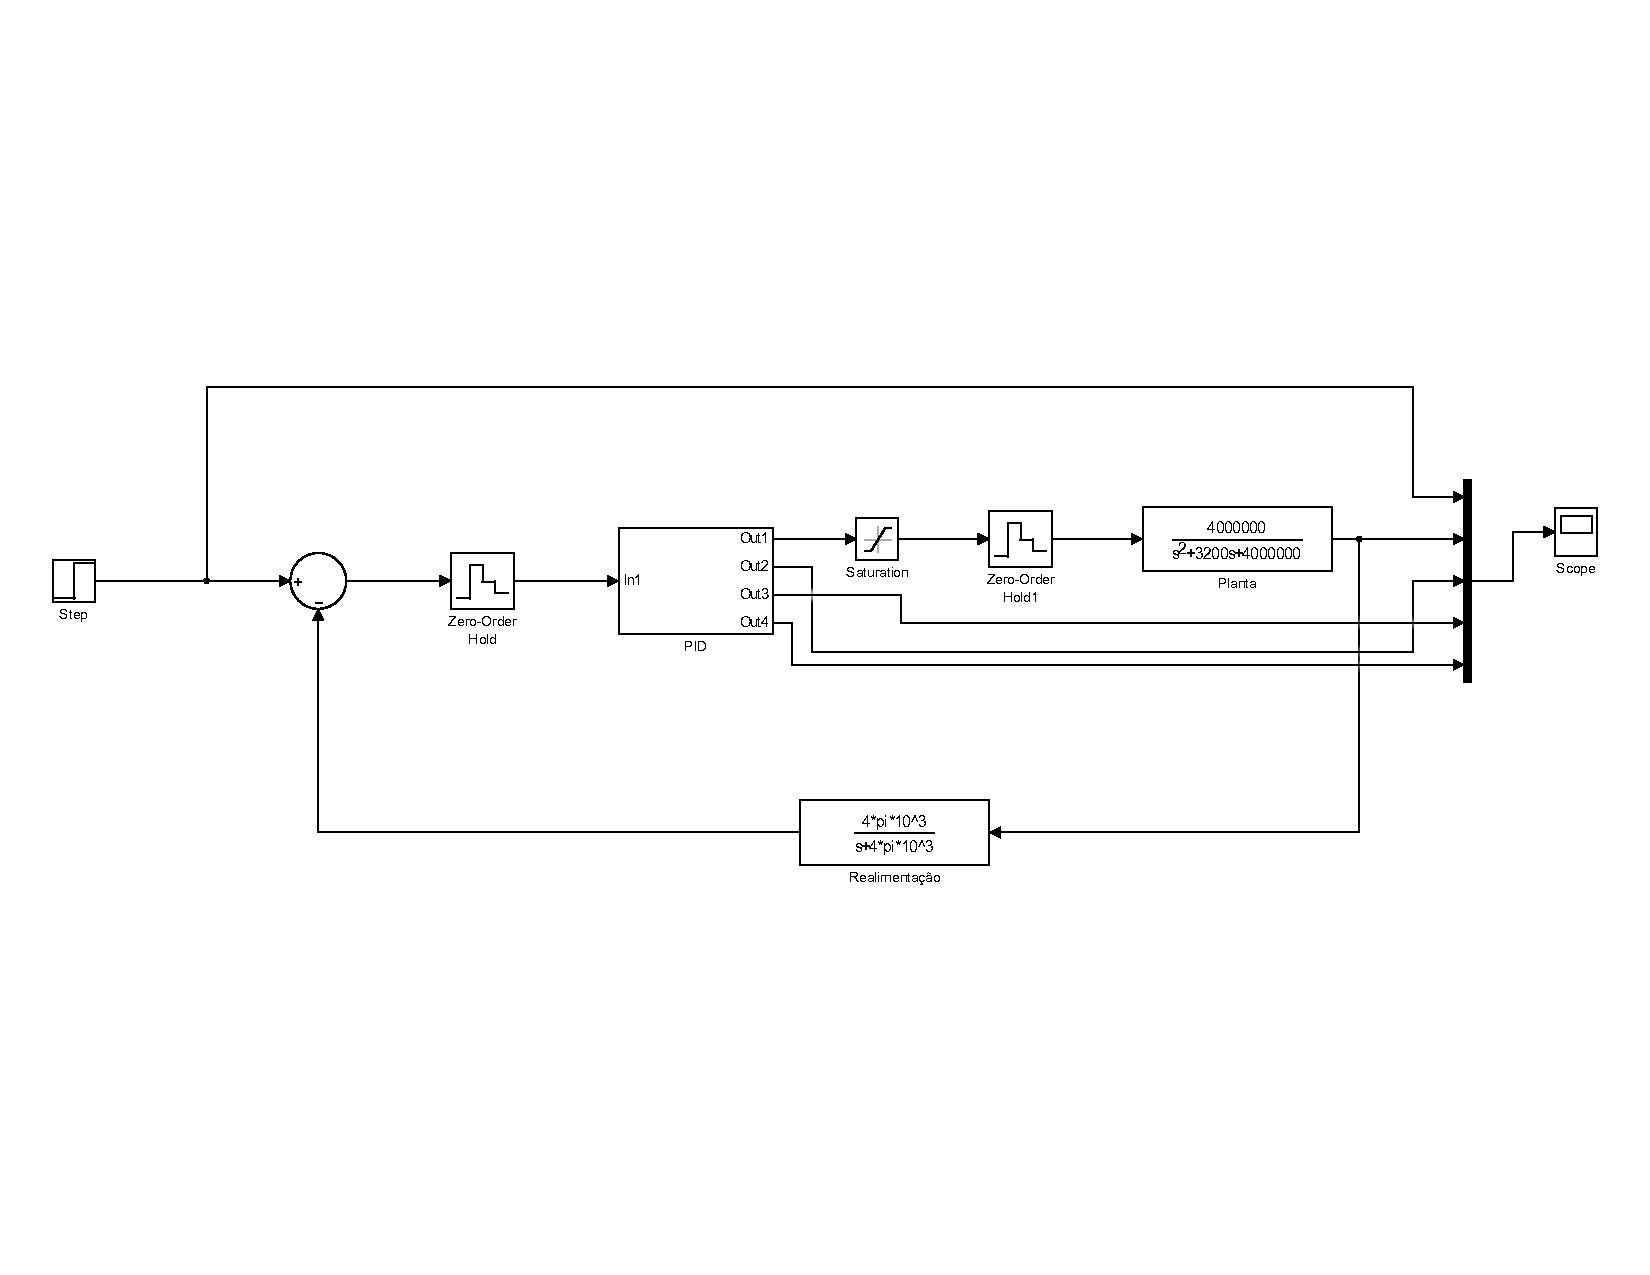
\includegraphics[scale = .4]{Imagens/Exercicio1_PID_SimulinkII.pdf}
		\caption{Diagrama de Blocos Exercício 1}
		\label{fig:Exercicio1_PID_SimulinkII}
	\end{figure}
	
	 A Figura \ref{fig:Exercicio1_PID_Simulink} está apresentado o circuito PID implementado. Os valores $K_P$, $K_D$ e $K_I$ são obtidos a partir dos método de projeto Ziegler-Nichols usando o procedimento 2. Ou seja foi obtido um ganho critico em malha fechada de modo que provoque um sinal de saída com oscilações constantes, e com base neste ganho e no período das oscilações constantes se defini os valores dos ganhos do PID.
	
	\begin{figure}[H]
		\centering
		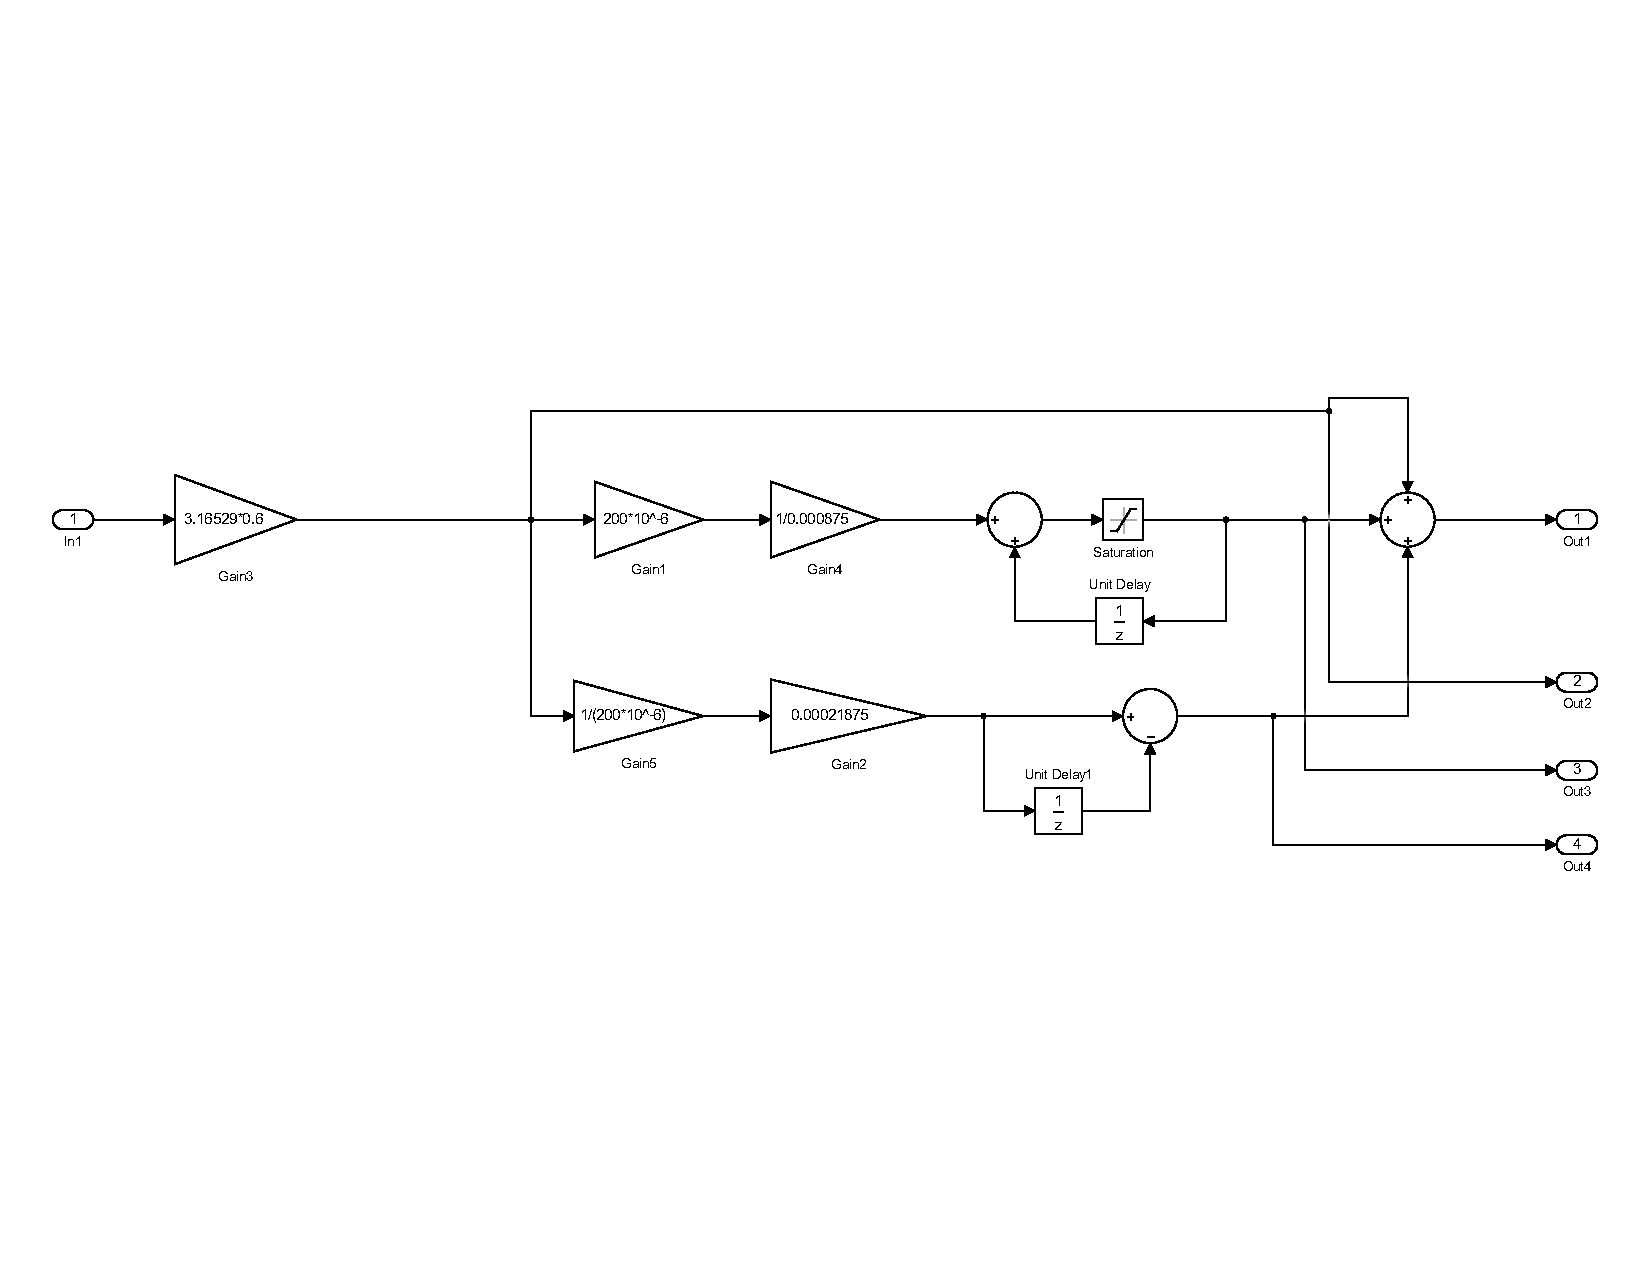
\includegraphics[scale = .4]{Imagens/Exercicio1_PID_Simulink.pdf}
		\caption{Diagrama de Blocos Exercício 1 - PID}
		\label{fig:Exercicio1_PID_Simulink}
	\end{figure}
	
	A Figura \ref{fig:PIDExercicioI} apresenta o resultado do circuito deste exercício simulado. As curvas contidas na Figura \ref{fig:PIDExercicioI} são referentes aos 5 sinais na entrada do bloco \emph{scope}, sendo: curva em amarelo representa o sinal de referência, curva em roxo representa a  resposta do sistema em malha fechada com PID, curva em azul a ação proporcional do PID, curva em vermelho a ação integrativa do PID e por fim a curva verde representa ação derivativa do PID.
	
	\begin{figure}[H]
		\centering
		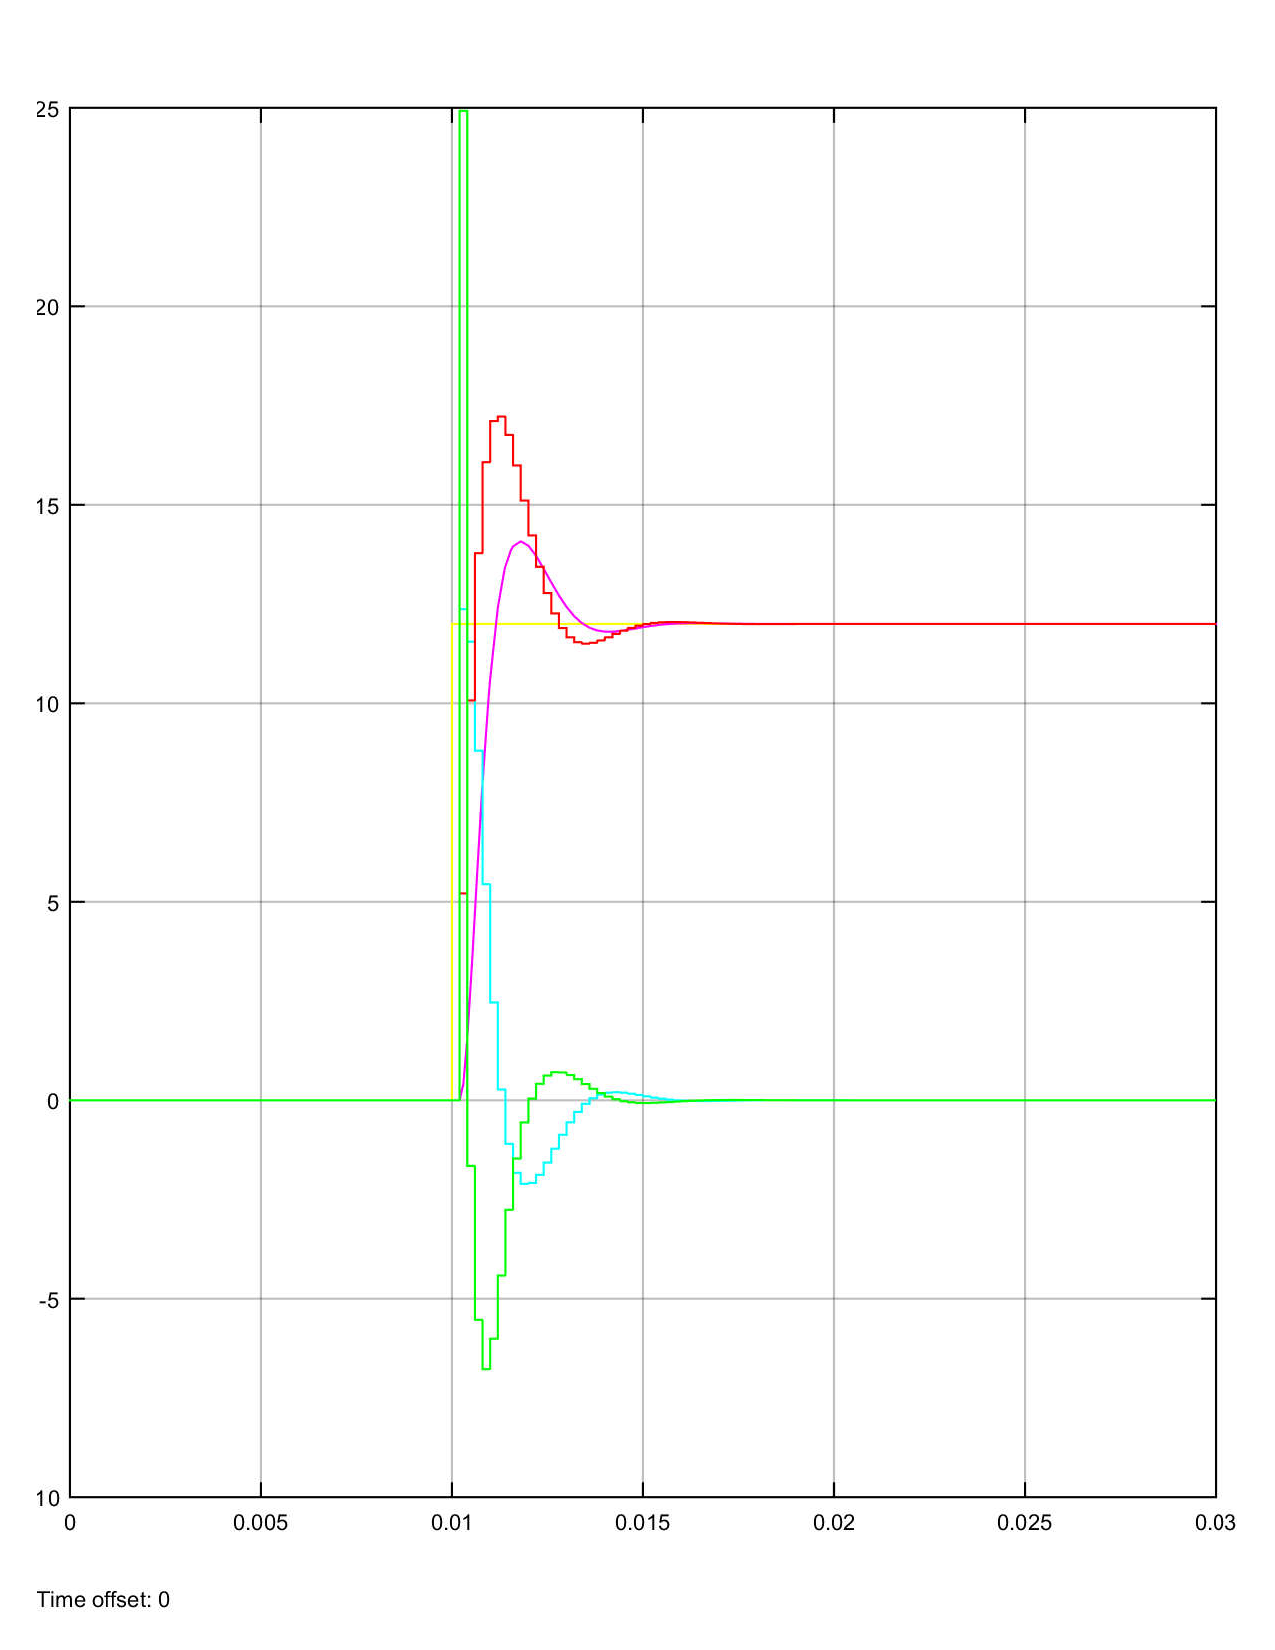
\includegraphics[scale = .4]{Imagens/PIDExercicioI.pdf}
		\caption{Resultado da Simulação do Exercício 1 - PID}
		\label{fig:PIDExercicioI}
	\end{figure}
	
	
\subsection{Exercício 2}
	Para a obtenção da função transferência do PID de tempo discreto usando o método de discretização \emph{Forward} se parte da equação básica do PID, definida pela Equação \ref{PIDEmTempo}.
	
	\begin{equation}
		u(t) = K \left( e(t) + \frac{1}{T_{i}} \int_0^t e(t) dt + T_d \frac{d}{dt} e(t) \right) 
		\label{PIDEmTempo}
	\end{equation}
	
	Seguindo a discretização, tornando $u_k = u(k)$ é possível aproximar a parcela de erro pela Equação \ref{erro}, a parcela integral pela Equação \ref{integral}, proveniente da discretização \emph{Forward}. E por fim a parcela derivativa pela Equação \ref{derivada}.
	
	\begin{equation}
		e(t) \rightarrow e_k
		\label{erro}
	\end{equation}
		
	\begin{equation}
		\int_0^t e(t) dt \rightarrow \sum_{i=0}^{k} e_i T
		\label{integral}
	\end{equation}
	
	\begin{equation}
		\frac{d}{dt} e(t) \rightarrow \frac{e_k - e_{k-1}}{T}
		\label{derivada}
	\end{equation}
	
	Logo pode-se definir a forma discreta do PID pela Equação \ref{PIDDiscreto}.
	 
	\begin{equation}
	u_k = K \left( e_k + \frac{T}{T_i} \sum_{i=0}^{k} (e_i) + \frac{T_d}{T}(e_k - e_{k-1})\right)
	\label{PIDDiscreto}
	\end{equation}
	
	Para que se possa eliminar o somatório da integral, que torna a implementação prática inaplicável, pode-se utilizar a transformada \emph{Z}. Logo pelas Equações \ref{transformadaZ1}, \ref{transformadaZ2} e \ref{transformadaZ3}.
	
	\begin{eqnarray}
		Z \{ e_k \} = E(z) \\
		Z \{ K \cdot e_k \} = K \cdot E(z)
		\label{transformadaZ1}
	\end{eqnarray}
	
	\begin{eqnarray}
		Z \{ e_{k-1} \} = z^{-1} E(z) \\
		Z \{ K_D ( e_k - e_{k-1}) \} = K_D(1-z^{-1}) E (z)
		\label{transformadaZ2}
	\end{eqnarray}
	
	\begin{eqnarray}
		Z \left\{ \sum_{i=0}^{k} f_i \right\} = \frac{1}{1 - z^{-1}} Z{f_i} \\
		Z \left\{ K_I \sum_{i = 0}^{k} e_i \right\} = K_I \frac{1}{1 - z^{-1}} E(z) \\
		\label{transformadaZ3}		
	\end{eqnarray}
	
	Logo temos a transformada Z para o PID se torna a Equação \ref{transformadaPIDZ}.
	
	\begin{equation}
		U(z) = K \left( E(z) + \frac{T}{T_i} \frac{1}{1 - z^{-1}} E(z) \frac{T_d}{T} (1 - z^{-1}) E(z) \right)
		\label{transformadaPIDZ}
	\end{equation} 
	
	Por fim tem-se pela propriedade do deslocamento a Equação \ref{PIDFinal}, que defini a equação discretizada do PID.
	
	\begin{eqnarray}
		u_P (k) = K_P~e(k) \\
		u_I (k) = K_I~e(k) + u_I~(k-1) \\
		u_D (k) = K_D~(e(k) - e(K - 1)) \\
		u_{PID} = u_P(k) + u_I (k) + u_D(k)
		\label{PIDFinal}	
	\end{eqnarray}
	
	Logo para se repetir o mesmo procedimento feito no exercício 2 aplicando a função do PID discretizada utilizando o método de \emph{Forward}  para parcela integral basta apenas
	modificar o valor do ganho $K_I$, já que ele é o único fator modificado pela mudança no método de discretização da integral. Portanto a figura \ref{fig:PIDExercicioII} apresenta o resultado da simulação do exercício 2, sendo que as curvas contidas nesta figura tem a mesma representação daquelas contidas  na Figura \ref{fig:PIDExercicioI}. 
	
	\begin{figure}[H]
		\centering
		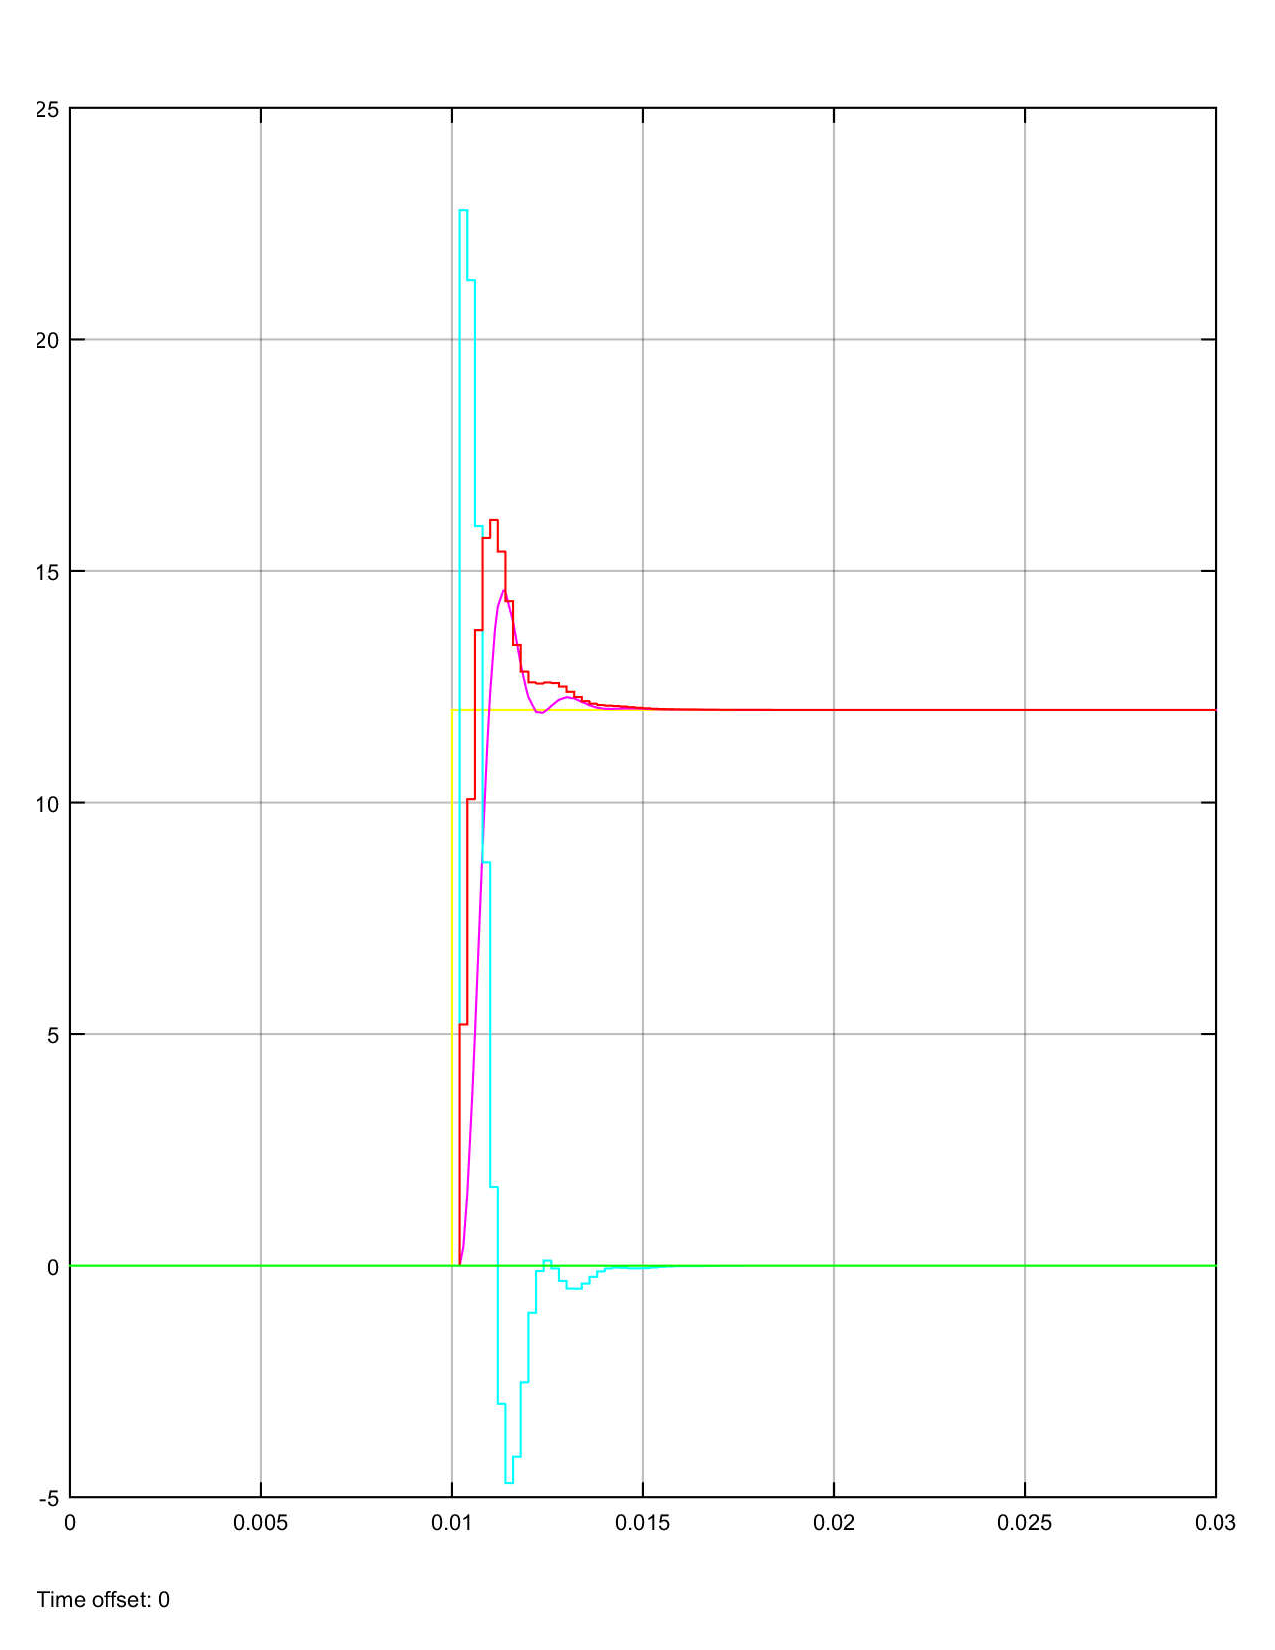
\includegraphics[scale = .4]{Imagens/PIDExercicioII.pdf}
		\caption{Resultado da Simulação do Exercício 2 - PID}
		\label{fig:PIDExercicioII}
	\end{figure}
	
	Os valores de $K$, $T_i$ e $T_d$ continuam sendo os mesmo daqueles usados no Exercício 1, sendo que o que muda neste exercício é a equação que defini a parcela $K_i$.
	
	\subsection{Exercício 3}
	
	Para a resolução do Exercício 3 é implementado em Matlab o código abaixo:
	\lstinputlisting{Arquivos_tex/Aula_6.m}
	
	O resultado desta simulação esta expressa na Figura \ref{fig:Exercicio3}.  
	
	\begin{figure}[H]
		\centering
		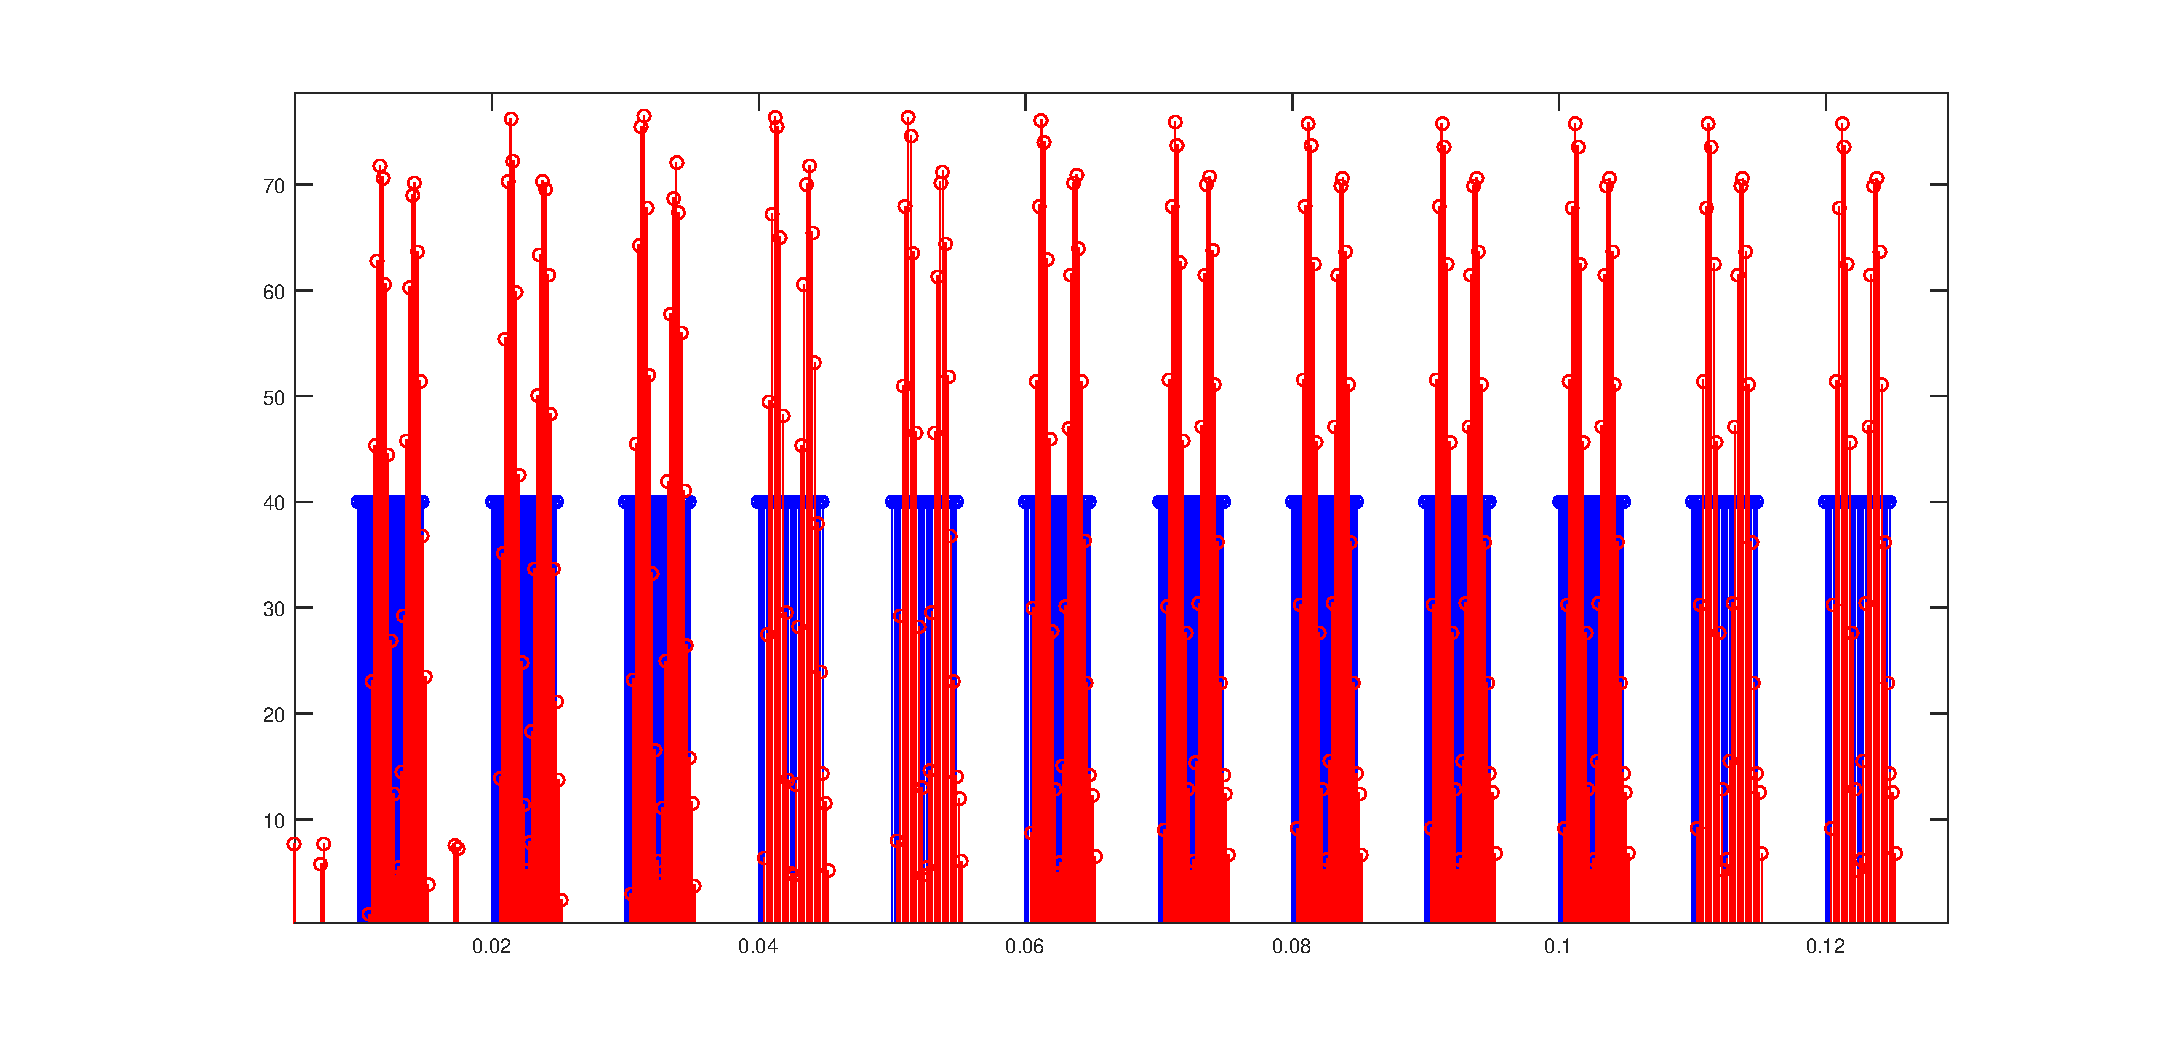
\includegraphics[scale = .4]{Imagens/ExercicioIII.eps}
		\caption{Simulação Exercicio 3 - Resposta em Malha Fechada}
		\label{fig:Exercicio3}
	\end{figure}